% GroundLM @ EMNLP 2026 submission.
% Uses the ACL template: drop acl.sty, acl_natbib.bst (and optionally
% ACL-style.sty) from https://github.com/acl-org/acl-style-files into this dir.
\documentclass[11pt]{article}
\usepackage[review]{acl}          % use [final] for camera-ready
\usepackage{times}
\usepackage{latexsym}
\usepackage[T1]{fontenc}
\usepackage[utf8]{inputenc}
\usepackage{microtype}
\usepackage{amsmath,amssymb}
\usepackage{booktabs}
\usepackage{graphicx}
\usepackage{enumitem}
\emergencystretch=1.5em   % avoid overfull hboxes in the narrow ACL columns

\title{A Support--Faithfulness Contrast Aligns Across Model Families\\
up to a Linear Map but Does Not Transfer to Real Hallucinations:\\
A Matched-Pair Study}

\author{Anonymous ACL submission}

\begin{document}
\maketitle

\begin{abstract}
Internals-based, reference-free hallucination detection treats ``context-faithfulness''
---is an answer entailed by the provided context?---as a linear direction in the
residual stream. But in the standard extractive setup, faithfulness is almost
perfectly correlated with \emph{lexical overlap} (whether the answer string occurs
in the context, $r{=}0.99$ in our data), so an apparent ``grounding probe'' may be a
string-matching detector. We introduce a matched \textsc{Support}$\times$\textsc{Overlap}
construction that decouples the two ($r{=}0.50$ on its model-free cells), including a
wrong-question trap on which an off-the-shelf NLI model is fooled ${\sim}25\%$ of the
time. With this control, on four instruction-tuned families (Llama-3.1-8B,
Qwen2.5-7B, Mistral-7B, Gemma-2-9B), we report: (i)~a mid-layer context-grounding
signal \emph{does} exist beyond lexical overlap---within the answer-present stratum,
where overlap is held constant, support is decodable at AUROC~$0.87$ (raw) and
$0.72$--$0.78$ after purging model confidence---though by construction this stratum
cannot separate grounding from factoid-correctness, so we make no claim of a grounding
axis geometrically distinct from factuality. (ii)~This direction \emph{aligns across
the four families up to a linear map}: an orthogonal-Procrustes map transports it
nearly collinear with each family's native direction (cosine~${\approx}0.98$, vs.\
${\approx}0.01$ for a random direction through the same map), and far exceeds an
anchor-projection baseline; we rest this on the geometry rather than the
(ceiling-saturated) transferred-probe AUROC. (iii)~Yet the synthetic direction
\emph{does not} transfer to real hallucination detection: on RAGTruth it scores below
NLI, confidence, and lexical overlap among single-pass API-free baselines, and within
a task no internals- or NLI-based signal (including a sentence-level SummaC-style NLI
baseline) exceeds ${\approx}0.6$ AUROC---while overlap's apparent edge
($0.753$ pooled, $0.647$ macro) is largely a between-task base-rate artifact. Only an
in-domain probe trained on human labels recovers a usable signal ($0.77$--$0.82$ on
the three RAGTruth families; it exceeds a single-hypothesis NLI baseline but only ties
lexical overlap on one). Our contribution is
a confound-controlled methodology, a released wrong-question diagnostic, and a
cautionary result: a grounding direction identified on controlled stimuli is real and
portable, but is not, by itself, a deployable hallucination detector. All experiments
are API-free and run on a single A100-40G.
\end{abstract}

\section{Introduction}
\label{sec:intro}

A grounded language model should answer from the \emph{provided context}, not from
its parametric memory or from surface cues. Reference-free, internals-based methods
operationalize this by reading a linear ``faithfulness'' or ``truth'' direction from
the residual stream
\citep{azaria2023saplma,marks2024geometry,burger2024truthuniversal,oneill2025singledirection},
an attractive recipe because it needs no external judge and costs roughly one
forward pass. Two distinct notions are routinely conflated under this banner:
\emph{parametric-factuality}---is a claim true in the model's memory?---and
\emph{context-faithfulness}---is a claim entailed by the given context? Recent work
treats both as activation objects and asks how they relate \citep{wang2025space},
but samples the two notions from \emph{different} datasets, so any measured geometry
is confounded with topic and lexicon.

We identify a sharper confound that undermines the faithfulness side specifically.
In the standard extractive QA setup used to build such probes (e.g.\ entity-swap
contexts \citep{longpre2021nqswap}), an answer is context-faithful \emph{iff} the
answer string occurs in the context. Faithfulness is therefore almost perfectly
correlated with \emph{lexical overlap} ($r{=}0.99$ in our data), and a probe that
appears to read ``grounding'' may simply detect string copying. Indeed, after
regressing out lexical overlap, an apparently excellent grounding probe collapses
to chance.

\paragraph{A matched control.}
We introduce a \textsc{Support}$\times$\textsc{Overlap} construction
(\S\ref{sec:construction}) that crosses semantic support with lexical presence in a
balanced $2\times2$. Two cells are model-free: a \emph{wrong-question trap}, where
the answer is present but answers a different question (supported${=}$no,
overlap${=}$yes), and the usual unsupported-absent cell; a paraphrase cell closes
the design. This drops $\mathrm{corr}(\textsc{support},\textsc{overlap})$ from
$0.99$ to $0.50$, and---tellingly---an off-the-shelf NLI model is fooled by the
clean wrong-question trap ${\sim}25\%$ of the time, confirming that lexical overlap
misleads even ``gold'' entailment checks.

\paragraph{Contributions.}
With this control we run a careful study across four model families
(Llama-3.1-8B, Qwen2.5-7B-Instruct, Mistral-7B-v0.3, Gemma-2-9B). We report two
positive results and two honest negatives.
\begin{enumerate}[leftmargin=1.4em,itemsep=1pt,topsep=2pt]
  \item \textbf{An overlap-independent support signal (\S\ref{sec:c1}).} Within the
    answer-present stratum (lexical overlap held constant), support is decodable on
    all four families: on the collision-free cells the raw within-stratum AUROC is
    near-ceiling (${\approx}0.99$) and stays at $0.76$--$0.88$ after purging model
    confidence, under item-grouped cross-validation. We are explicit about two limits.
    (i)~Within this stratum the contrast varies \emph{only the question}, so the
    signal may reflect question--answer appropriateness rather than use of the
    context; a question-fixed cross-strata control (\S\ref{sec:c1}) bounds how much is
    context-driven.
    (ii)~Support and our \emph{synthetic} factuality label are identical here by
    construction, so this isolates the signal from \emph{lexical overlap} but
    \emph{not} from factoid-correctness. We therefore claim a non-overlap
    support/appropriateness signal, not a grounding axis geometrically distinct from
    factuality.
  \item \textbf{Cross-family alignment up to a linear map (\S\ref{sec:c3}).} An
    orthogonal-Procrustes map carries the support direction between families so the
    transported direction is nearly collinear with the target family's \emph{native}
    direction (cosine ${\approx}0.98$, vs.\ ${\approx}0.01$ for a random direction
    through the same map), whereas an anchor-projection transfer reaches only $0.67$
    AUROC \citep{kim2026crossfamily}. The transferred-probe AUROC ($0.91$) equals the
    within-family bound but is ceiling-saturated, and signed map-aware nulls sit at
    chance ($0.51$); we therefore rest the claim on the cosine. Factuality, answer-length and overlap directions transport identically while a
    confidence direction does not, indicating a shared stimulus-derived contrast
    rather than a grounding-specific axis; we claim no
    universality beyond these four $7$--$9$B models \citep{puri2025atlas}.
  \item \textbf{No confidence asymmetry (\S\ref{sec:c2}).} Contrary to a natural
    hypothesis, softmax confidence and activation norm do not absorb the
    factuality axis more than the faithfulness axis; the effect is null.
  \item \textbf{Synthetic axes do not transfer to real hallucinations
    (\S\ref{sec:c4}).} Applied to RAGTruth \citep{niu2024ragtruth}, the
    controlled-stimulus support direction scores \emph{below} NLI, confidence, and
    lexical overlap among single-pass API-free baselines; within a task no internals-
    or NLI-based signal---including a sentence-level SummaC-style NLI baseline---exceeds
    ${\approx}0.6$ AUROC, and even lexical overlap, the strongest baseline, reaches only
    macro $0.647$. An in-domain probe trained on RAGTruth human
    labels recovers a usable signal ($0.77$--$0.82$ on the three RAGTruth families;
    exceeds a conservative single-hypothesis NLI baseline but ties lexical overlap on
    Qwen), so a real support signal exists in the internals but is a \emph{different
    direction} from the synthetic axis and needs in-domain annotation.
\end{enumerate}
The takeaway for the ``faithful and efficient'' agenda is cautionary but useful:
internals-based support contrasts identified on controlled data are real and
remarkably portable across model families (though not grounding-specific), yet are
\emph{not}, by themselves, deployable hallucination detectors---on real data, lexical
overlap still dominates.

\section{Related Work}
\label{sec:related}

\paragraph{Geometry of truth and faithfulness.}
Linear ``truth'' directions are decodable from activations
\citep{azaria2023saplma,marks2024geometry} and partly shared across models
\citep{burger2024truthuniversal}, but are task-dependent and often fail to transfer
across tasks \citep{azizian2025orthogonal,bao2025probing}. \citet{wang2025space}
treat factuality and faithfulness hallucinations as activation subspaces and argue
they overlap; crucially they draw the two notions from different corpora, leaving
the geometry confounded with surface form. \citet{adarsh2026context} study how a
single truth vector rotates when context is added. We instead hold the two notions
on \emph{matched} stimuli and control lexical overlap explicitly; we note, however,
that our factuality label is a synthetic gold-answer relabeling rather than a
parametric memory-truth probe, so we engage this line methodologically without
claiming to adjudicate whether factuality and faithfulness share a direction.

\paragraph{Knowledge conflict and source attribution.}
Probes can detect knowledge conflict and predict which source a model follows
\citep{zhao2024residualconflict,sun2025redeep,brink2026attribution}. These are
behavioral/source signals; we ask whether a \emph{content} grounding axis exists
that is not reducible to lexical overlap.

\paragraph{Cross-model transfer.}
Linear concept directions can be aligned across models via orthogonal Procrustes
\citep{puri2025atlas} or anchor projection \citep{kim2026crossfamily}. We apply both
to a support direction; Procrustes renders it nearly collinear with the target's
native direction (cosine ${\approx}0.98$) whereas anchor projection does not.

\paragraph{Reference-free hallucination detection.}
NLI/entailment and alignment scores \citep{zha2023alignscore}, single residual
directions \citep{oneill2025singledirection}, confidence/correctness probes
\citep{cho2026confidencemanifold,noanswer2025}, and faithfulness-aware UQ
\citep{fadeeva2025franq} all target RAG faithfulness. We use NLI, confidence, and
lexical overlap as baselines on RAGTruth and find our controlled-stimulus axis does
not beat them.

\section{The \textsc{Support}$\times$\textsc{Overlap} Construction}
\label{sec:construction}

We build matched statements from NQ-Swap \citep{longpre2021nqswap}, which provides,
per question $q$, a gold answer $a_{\mathrm{true}}$ supported by an original context
$c_{\mathrm{org}}$ and a substituted entity $a_{\mathrm{swap}}$ supported by an
entity-swapped context $c_{\mathrm{sub}}$. We define two bits per (context, answer):
\textsc{Support}~$S$ (does the given context entail the asserted answer for the asked
question?) and \textsc{Overlap}~$O$ (does the answer string occur in the context?).
The $2{\times}2$ design has four cells, of which we realize three (cell~B is
unrealized in this release; see below):
\begin{center}\small
\begin{tabular}{@{}llcc@{}}
\toprule
cell & (question, context, answer) & $S$ & $O$ \\
\midrule
A & $(q,\ c_{\mathrm{org}},\ a_{\mathrm{true}})$ & 1 & 1 \\
B & $(q,\ \mathrm{paraphrase}(c_{\mathrm{org}}),\ a_{\mathrm{true}})$ & 1 & 0 \\
C & $(q',\ c_{\mathrm{org}},\ a_{\mathrm{true}})$ & 0 & 1 \\
D & $(q,\ c_{\mathrm{sub}},\ a_{\mathrm{true}})$ & 0 & 0 \\
\bottomrule
\end{tabular}
\end{center}
Cell~C is a \emph{wrong-question trap}: $a_{\mathrm{true}}$ is present in
$c_{\mathrm{org}}$ but is offered as the answer to a different question $q'$ (the
next item's question). Cell~B paraphrases $c_{\mathrm{org}}$ so the answer is
entailed but not copied (open instruct model, kept only if token-overlap${\le}0.34$
and an NLI model still entails it); in this release cell~B has \emph{zero} yield, so
all reported analyses use the model-free cells A/C/D with
$\mathrm{corr}(S,O){=}0.50$ ($0.57$ after removing the donor-collision items below; an
orthogonalized $\mathrm{corr}{\approx}0$ design would require cell~B). One caveat in cell~C: NQ-Swap dev has only $418$ distinct questions
over $1{,}200$ items, so for $278$ items ($23.2\%$) the donor $q'$ is string-identical
to $q$ and $a_{\mathrm{true}}$ \emph{does} answer it; we flag these
\emph{donor-collision} items and report cell-C results with them removed (the full
construction will dedup $q'{\neq}q$). On \emph{clean} cell~C an open NLI model
\citep{he2023debertav3} still rates $25.5\%$ of unsupported-but-present items as
``supported'' (mean entailment $0.31$, vs.\ $0.74$ for cell~A and $0.18$ for cell~D);
the raw $37.6\%$ rate is inflated by the collisions, which NLI entails $77.7\%$ of the
time (correctly). Lexical overlap thus misleads ``gold'' entailment even after the
label error is purged (Fig.~\ref{fig:decoupling}).

\begin{figure*}[t]\centering
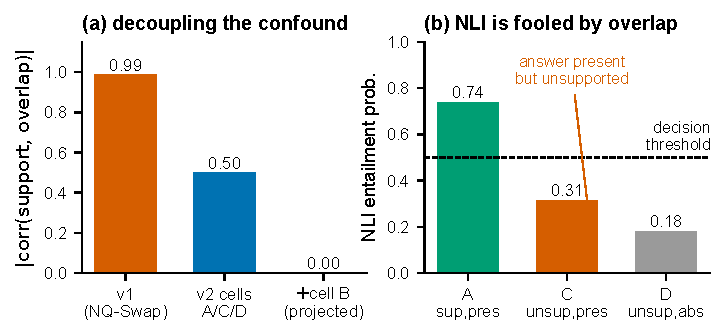
\includegraphics[width=0.86\textwidth]{figs/fig_decoupling.pdf}
\caption{\textbf{Partially decoupling support from lexical overlap.} (a)~The matched
construction drops $|\mathrm{corr}(\textsc{support},\textsc{overlap})|$ from $0.99$
(extractive NQ-Swap) to $0.50$ (model-free cells A/C/D), and would reach $\approx 0$
with the paraphrase cell~B (projected; cell~B has zero yield in this release).
(b)~Mean NLI entailment by \emph{clean} cell: on the wrong-question trap~(C), where the
answer is present but unsupported, NLI is still pulled toward ``supported.''}
\label{fig:decoupling}
\end{figure*}

\section{Probing, Separability, and Transfer}
\label{sec:method}

\paragraph{Directions.}
For a (model, layer) we extract last-token residual states $X$ over the asserted
answer span (one forward pass, bf16, left-padded). A \textsc{Support} direction
$d_S$ and \textsc{Factuality} direction $d_F$ are mass-mean
(difference-of-means) estimates \citep{marks2024geometry}; signed projections
$X d$ are the probe scores. We report layer-wise cross-validated AUROC under
\emph{GroupKFold on \textsc{item\_id}}: because cells A/C/D of an item reuse the
same context, an ungrouped split would leak near-duplicate rows across folds, so
all statements of one item are kept in a single fold. Axis polarity is fixed on
the \emph{train} fold; the test projection is scored as-is (no
$\max(\mathrm{AUC},1{-}\mathrm{AUC})$ flip), so a non-predictive direction
correctly averages to $0.5$ rather than being floored above it. All point
estimates carry item cluster-bootstrap 95\%\,CIs.

\paragraph{Overlap control.}
To test grounding \emph{beyond} overlap we (i) restrict to the answer-present
stratum $O{=}1$ (cells A vs.\ C), where lexical presence is constant, and
(ii) residualize $X$ on surface covariates (overlap, length) before re-probing.

\paragraph{Null-calibrated separability.}
We treat each notion as an undirected axis and measure the acute angle
$\angle(d_S,d_F)$. Significance is assessed against a within-notion null built by
splitting one notion's data in half and measuring the half-vs-half angle; a
permutation test with $n_{\mathrm{null}}{=}10{,}000$ draws gives $p$. We report
the resolution bound $p{<}1/n_{\mathrm{null}}{=}10^{-4}$ rather than $p{=}0$ when
no null draw exceeds the observed angle, and state that the test is run per family
at the a-priori mid layer (four families $\times$ one layer).

\paragraph{Confidence purge.}
We regress each hidden dimension on confidence covariates (max-softmax, answer
log-prob, activation norm) and re-probe the residual, reporting the fraction of
probe signal absorbed per axis.

\paragraph{Cross-family transfer.}
Families differ in hidden size, so we fit a semi-orthogonal Procrustes map between
two models' residual spaces on a shared calibration split, transport a
source-trained probe, and measure target AUROC. The calibration/evaluation split
is a \emph{GroupKFold on \textsc{item\_id}} (items in the calibration set are
disjoint from the evaluation set), so the map is never fit and tested on
near-duplicate rows of the same item; transported-probe polarity is fixed on the
target calibration fold. We compare to an unconstrained ridge map, the
anchor-projection ACS baseline \citep{kim2026crossfamily}, a within-family upper
bound, and a random-direction floor (also scored without the polarity flip, so it
sits at chance rather than being inflated above $0.5$).

\section{Experiments}
\label{sec:experiments}

\paragraph{Setup.}
Four instruction-tuned families: Llama-3.1-8B, Qwen2.5-7B, Mistral-7B-v0.3,
Gemma-2-9B. CtrlPairs: $1{,}200$ NQ-Swap items $\to 3{,}593$ matched statements
(cells A/C/D). RAGTruth: $2{,}000$ test responses with response-level hallucination
labels \citep{niu2024ragtruth}. Baselines: NLI (DeBERTa-v3-base-mnli-fever-anli \citep{he2023debertav3}) in two
variants---(i)~\emph{whole-response}: a single (context, declarativized-answer)
entailment query (deliberately simple and conservative for multi-sentence responses);
and (ii)~\emph{sentence-level}, a SummaC-style decomposition \citep{laban2022summac}
that entailment-checks each response sentence against every context sentence, takes the
max over context, and aggregates over response sentences by mean (SummaC-ZS) or min
(for tractability we cap context at $60$ sentences and pairs at $256$ tokens, which can
only lower SummaC and is thus conservative)---plus max-softmax confidence and lexical
overlap. Everything is API-free; the NLI baselines use the small DeBERTa model and all
activation extraction runs on one A100-40G.

\subsection{A support signal beyond lexical overlap}
\label{sec:c1}
\paragraph{Leakage-controlled protocol.}
Cells A/C/D of an item share the original context $c_{\mathrm{org}}$ verbatim
(A and C are the same context with a different question), so a plain row-level
split would place near-duplicate rows of one item on both sides of the
train/test boundary. We therefore use \emph{GroupKFold on \textsc{item\_id}}
throughout: all statements derived from one NQ-Swap item fall in the same fold,
for both the C1 cross-validation and the Procrustes calibration/evaluation split
(\S\ref{sec:c3}). We resolve each estimated axis's sign on the \emph{train} fold
only (never on the test fold), so test AUROC can fall below $0.5$ and is not
floored by a $\max(\mathrm{AUC},1{-}\mathrm{AUC})$ flip. To avoid selecting the
layer on the very number we report, we fix the analysis layer \emph{a priori} at
relative depth $0.5$ (the nearest cached layer to $0.5\,L_{\mathrm{tot}}$:
$L{=}14/16/16/21$ for Qwen/Mistral/Llama/Gemma), matching the relative-depth
convention already used for C3/C4 and for Fig.~\ref{fig:c1layers}; we additionally
report the mean$\pm$sd across the mid-layer band ($0.4$--$0.6$ depth) to show the
result is not a single-layer artifact. Confidence intervals are item cluster
bootstraps (resampling \textsc{item\_id} with replacement).

Table~\ref{tab:c1} reports support decodability within the answer-present stratum
$O{=}1$ (cells A vs.\ C), where lexical overlap is held constant, on the
\emph{collision-free} cells: we drop the $23.2\%$ of cell-C items whose donor question
is string-identical to the original (\S\ref{sec:construction}), which would otherwise
mislabel genuinely-supported items as unsupported. Three observations bound the
interpretation. First, the raw within-stratum AUROC is \emph{near-ceiling}
($0.99$; $0.988$--$0.999$ across families): once mislabels are removed, $A$ and $C$ are
almost perfectly separable. We read this less as strong grounding than as evidence
that the contrast is \emph{easy}---within $O{=}1$ it varies \emph{only the question}
(context and answer are fixed), so a probe can in principle separate $A$ from $C$ by
question--answer appropriateness without using the context. Second, the operative
confound is \emph{model confidence} (overlap and answer length are uninformative here,
AUROC~$0.500$): answer log-prob and NLI separate $A$ from $C$ on their own, so we
residualize the hidden states on log-prob and max-softmax; the support contrast then
falls to $0.76$--$0.88$, which we take as the primary confound-controlled estimate.
Third, a cross-strata control that \emph{fixes the question} (train $A$ vs.\ $D$, where
only the context changes; evaluate $A$ vs.\ $C$) transfers at $0.66$--$0.88$, weakest
on Qwen: a context-driven component is present, but the gap to the raw ceiling is
consistent with a residual question--answer-compatibility component that this matched
design cannot rule out. Finally, support and our \emph{synthetic} factuality label are
\emph{identical} within $O{=}1$ by construction (they diverge only in the
answer-absent cell~D), so this isolates the signal from \emph{lexical overlap} but
\emph{not} from factoid-correctness; we claim a non-overlap support/appropriateness
signal, not a grounding axis geometrically distinct from factuality. The decisive
control---re-extracting $A$ vs.\ $C$ with the context \emph{removed} (question$+$answer
only) or replaced by an unrelated passage---would separate context use from
question--answer compatibility directly; pending that no-context ablation we bound the
context's contribution only via the cross-strata control above ($0.66$--$0.88$).

\begin{table}[t]\centering\small
\setlength{\tabcolsep}{3.5pt}
\begin{tabular}{@{}lcccc@{}}
\toprule
model & $L$ & supp$_{O=1}$ & {\footnotesize$+$conf} & {\footnotesize cross} \\
\midrule
Qwen2.5 & 14 & 0.988 & 0.757 & 0.660 \\
Mistral & 16 & 0.996 & 0.878 & 0.870 \\
Llama   & 16 & 0.997 & 0.784 & 0.876 \\
Gemma   & 21 & 0.999 & 0.806 & 0.827 \\
\bottomrule
\end{tabular}
\caption{\textbf{C1 (confound-controlled, collision-free).} Layer fixed a priori at
relative depth $0.5$; GroupKFold on \textsc{item\_id}; polarity resolved on the train
fold; donor-collision cell-C mislabels removed (\S\ref{sec:construction}; $n_A{=}1200$,
$n_C{=}922$). supp$_{O=1}$ is grouped-CV support AUROC within the answer-present
stratum---near-ceiling once mislabels are removed, because the contrast varies only the
question and is easily separable. \emph{$+$conf}: after residualizing the hidden states
on confidence (log-prob, max-softmax)---our primary estimate. \emph{cross}: train $A$
vs.\ $D$ (question fixed, only context changes), evaluate $A$ vs.\ $C$. Within $O{=}1$
support and the synthetic factuality label coincide, so we make no distinctness claim.}
\label{tab:c1}
\end{table}

\begin{figure*}[t]\centering
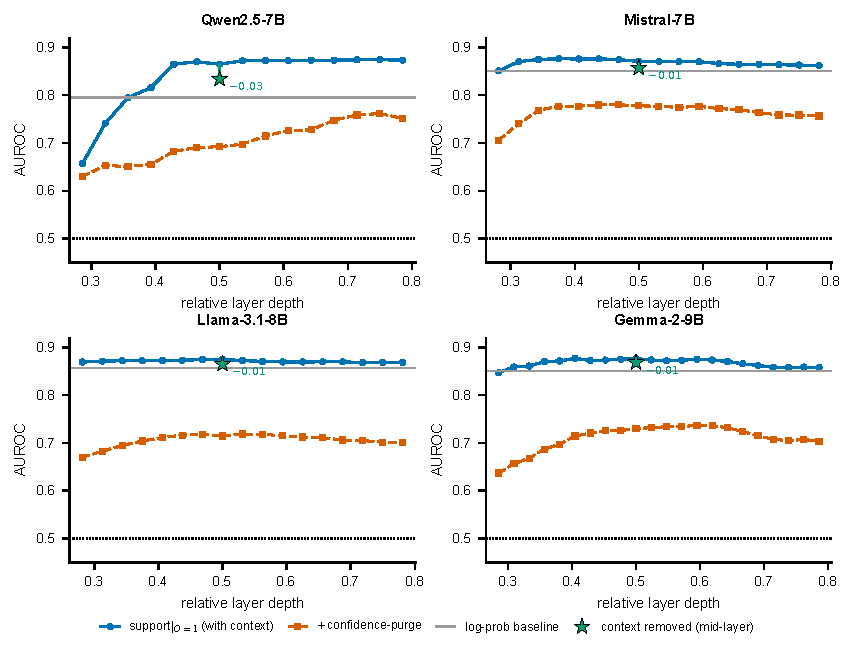
\includegraphics[width=0.9\textwidth]{figs/fig_c1_layers.pdf}
\caption{\textbf{A support signal beyond overlap, peaking mid-layer.}
Cross-validated AUROC vs.\ relative layer depth for support within the
answer-present stratum ($O{=}1$, where overlap is uninformative), support after
removing surface covariates, and factuality. The overlap-independent support
signal is high and stable through mid layers on all four families.}
\label{fig:c1layers}
\end{figure*}

\subsection{No confidence asymmetry}
\label{sec:c2}
We hypothesized that confidence absorbs the factuality axis more than the
faithfulness axis, which would offer a way to separate them. The measured asymmetry
is small and inconsistent in sign across the families and layers we examined (it does
not favour the factuality axis), so we report a null result and do not rely on
confidence-purging to distinguish the two notions.

\subsection{Matched-stimulus contrasts align across families up to a linear map}
\label{sec:c3}
We ask whether the support direction occupies the \emph{same} geometry across
families up to a linear map. The direct evidence is geometric: the Procrustes-mapped
source direction is nearly collinear with the target family's \emph{native} direction
(transported-to-native cosine $0.976$, range $0.95$--$0.99$ over the $12$ ordered
pairs; Table~\ref{tab:c3}), well above anchor projection. The cosine is far above its
null: a random or label-shuffled source direction transported through the \emph{same}
fitted map is essentially orthogonal to the native direction (cosine $0.01$ and $0.10$
respectively), so $0.976$ is not an artifact of the shared-stimulus geometry. We
deliberately do \emph{not} headline the transferred-probe AUROC ($0.906$): it equals
the within-family bound ($0.905$) and is therefore ceiling-saturated; scored with
polarity-honest (signed) AUROC, random and shuffled-label directions through the map
sit at chance ($0.51$/$0.51$). \textbf{This alignment is not specific to grounding.}
Transporting the \emph{factuality}, \emph{answer-length}, and \emph{lexical-overlap}
directions through the same maps gives cosines of $0.99$/$0.98$/$0.99$---as high as
support---whereas a purely model-internal \emph{confidence} direction transports at
only $0.50$ (and unstably, $0.04$--$0.90$ across pairs). So what aligns is any contrast
\emph{derived from the shared input stimuli}, a shared low-rank stimulus geometry, not
a grounding-specific axis; that confidence does \emph{not} align shows the alignment is
non-trivial but also that it carries no grounding-specific content. We therefore
conclude only that \emph{matched-stimulus contrasts---support among them---are linearly
alignable across these four $7$--$9$B families}, and avoid any claim of a
grounding-specific or near-lossless transfer.

\begin{table}[t]\centering\small
\setlength{\tabcolsep}{3.5pt}
\begin{tabular}{@{}lccccc@{}}
\toprule
axis & cosine & AUROC & within & rand-map & rand-lab \\
\midrule
\textsc{Support}    & \textbf{0.976} & 0.906 & 0.905 & 0.519 & 0.506 \\
\textsc{Factuality} & 0.989 & 0.915 & 0.911 & --- & --- \\
\midrule
\multicolumn{6}{@{}l}{\footnotesize\itshape nuisance directions:}\\
length     & 0.976 & --- & --- & --- & --- \\
overlap    & 0.992 & --- & --- & --- & --- \\
confidence & 0.504 & --- & --- & --- & --- \\
\bottomrule
\end{tabular}
\caption{\textbf{C3 (cosine-based, leakage-controlled).} Mean over the $12$
cross-family ordered pairs, GroupKFold on \textsc{item\_id}. \emph{cosine}:
transported-to-native cosine (the alignment evidence; non-saturating). A random /
label-shuffled source direction through the \emph{same} map has cosine only $0.01$ /
$0.10$ with the native direction. \emph{AUROC}/\emph{within}: transferred-probe vs.\
within-family AUROC---equal, hence ceiling-saturated. \emph{rand-map}/\emph{rand-lab}:
random / shuffled-label directions through the map, signed AUROC, at chance. Support,
factuality, answer-length and overlap directions all align at ${\approx}0.98$, while a
model-internal confidence direction does not ($0.50$): alignment is a generic property
of contrasts derived from the shared stimuli, not a grounding-specific axis.}
\label{tab:c3}
\end{table}

\begin{figure}[t]\centering
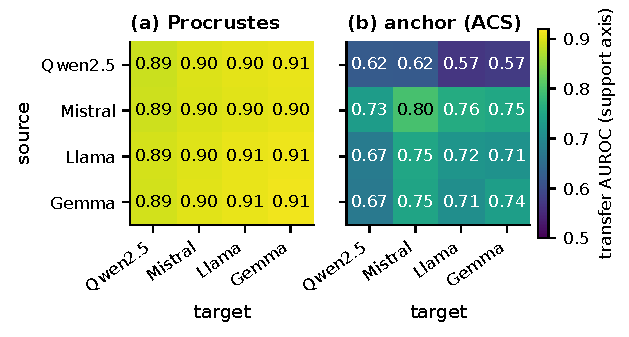
\includegraphics[width=\columnwidth]{figs/fig_c3_heatmap.pdf}
\caption{\textbf{Matched-stimulus contrasts align across families up to a linear map.}
Source$\to$target transfer AUROC of the support direction. (a)~Orthogonal Procrustes
is uniformly high on- and off-diagonal; we read this as alignment (cosine $0.98$,
Table~\ref{tab:c3}), not as lossless transfer, since the AUROC is ceiling-saturated.
(b)~Anchor projection (ACS) matches it only within-family and degrades sharply across
families.}
\label{fig:c3heatmap}
\end{figure}

\subsection{Synthetic axes do not transfer to real hallucinations}
\label{sec:c4}
We learn $d_S$ on CtrlPairs and apply it to the fixed RAGTruth responses (hidden states
extracted through that same model; the responses are RAGTruth's own, so the NLI and
overlap baselines are response-intrinsic and identical across the three models),
predicting the human faithfulness label (Table~\ref{tab:c4}). Here we keep the
\emph{support-polarity} sign fixed from CtrlPairs and score without the
test-fold flip, because flipping per-test inflates a near-chance axis; CtrlPairs
and RAGTruth share no items, so there is no leakage in this transfer. Scored
honestly, the label-free synthetic axis reaches only $0.54$--$0.66$\,AUROC
(and drops toward chance for the weakest family)---\emph{below} NLI ($0.673$),
model confidence ($0.62$--$0.72$), and plain lexical overlap ($0.753$), which is
the single best predictor on RAGTruth. Removing the polarity flip can only lower
these numbers, so the C4 negative is if anything understated by the original
table. Thus on real data overlap still dominates, and even NLI does not escape it.
A more sophisticated sentence-level NLI baseline (SummaC-style, max entailment over
context sentences) does no better: pooled $0.614$/$0.664$ and within-task macro
$0.596$/$0.579$ (mean/min), essentially tied with the whole-response NLI ($0.582$,
within sampling noise) and still well below overlap (Table~\ref{tab:c4_pertask})---consistent
with RAGTruth hallucinations often being abstractive or reasoning-level errors that
survive sentence-by-sentence entailment, on which a small off-the-shelf NLI model has
limited headroom.
An \emph{in-domain} probe ($5$-fold grouped-CV $L_2$-logistic on the same mid-layer
states, target${=}$human faithfulness label) does recover a usable signal:
AUROC $0.77$/$0.82$/$0.80$ for Qwen/Llama/Gemma (item-bootstrap $95\%$ CIs in
Table~\ref{tab:c4}). It exceeds our NLI baseline ($0.673$) on all three families---though that
baseline scores each multi-sentence response with a single whole-response entailment
check and is conservative (\S\ref{sec:experiments}); against the strong overlap
baseline ($0.753$) it wins on Llama and Gemma (paired bootstrap $p{<}0.001$) but only
ties on Qwen ($+0.01$, $p{=}0.17$). Residualizing lexical overlap out of the
features first drops it to $0.60$--$0.66$, so much of even this signal is overlap. A
real support signal therefore exists in the internals, but it is a \emph{different
direction} from the synthetic axis and is recoverable only with in-domain human
annotation.

\begin{table}[t]\centering\small
\setlength{\tabcolsep}{3.5pt}
\begin{tabular}{@{}lccc|cc@{}}
\toprule
 & \multicolumn{3}{c}{label-free} & NLI & overlap \\
model & synth-$d_S$ & conf & in-dom$^{\dagger}$ & & \\
\midrule
Qwen2.5 & 0.657 & 0.723 & 0.766 & 0.673 & 0.753 \\
Llama   & 0.591 & 0.623 & 0.816 & 0.673 & 0.753 \\
Gemma   & 0.541 & 0.686 & 0.800 & 0.673 & 0.753 \\
\bottomrule
\end{tabular}
\caption{\textbf{C4 (leakage-controlled).} RAGTruth hallucination detection
(AUROC; three families---Mistral's RAGTruth extraction OOM'd). The label-free
synthetic support axis (synth-$d_S$, support polarity
fixed from CtrlPairs, a-priori mid layer, scored without the test-fold flip) is
below NLI, confidence, and lexical overlap, and for the weakest family
(Gemma, $0.541$) is barely above chance. $^{\dagger}$in-domain probe uses RAGTruth
human labels (not label-free).}
\label{tab:c4}
\end{table}

\begin{figure}[t]\centering
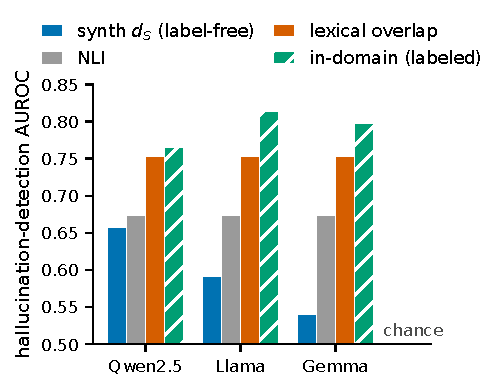
\includegraphics[width=0.92\columnwidth]{figs/fig_c4_ragtruth.pdf}
\caption{\textbf{The synthetic axis does not transfer to real hallucinations.}
On RAGTruth, the label-free synthetic support axis (ours) sits below NLI and below
plain lexical overlap, the strongest baseline; only an in-domain probe trained on
human labels beats NLI. Axis starts at chance ($0.5$).}
\label{fig:c4}
\end{figure}

\begin{table}[t]\centering\small\setlength{\tabcolsep}{3pt}
\begin{tabular}{@{}lcccc@{}}
\toprule
signal & Data2txt & QA & Summary & macro \\
\midrule
synth-$d_S$        & 0.541 & 0.611 & 0.658 & 0.604 \\
confidence         & 0.591 & 0.544 & 0.679 & 0.605 \\
NLI, whole-resp.   & 0.547 & 0.567 & 0.633 & 0.582 \\
NLI, sent.\ (mean) & 0.611 & 0.557 & 0.620 & 0.596 \\
NLI, sent.\ (min)  & 0.521 & 0.591 & 0.626 & 0.579 \\
overlap            & 0.605 & 0.686 & 0.649 & 0.647 \\
\midrule
in-domain$^{\dagger}$ & 0.742 & 0.721 & 0.679 & 0.714 \\
\midrule
faithful-rate & 0.357 & 0.823 & 0.795 & --- \\
\bottomrule
\end{tabular}
\caption{\textbf{C4, per task type.} Within-task RAGTruth AUROC (synth-$d_S$,
confidence, and in-domain are the mean over the three RAGTruth models; NLI and overlap
are response-intrinsic). The pooled numbers in Table~\ref{tab:c4} overstate every
signal because faithful base rates differ sharply across tasks (bottom row): overlap's
pooled $0.753$ falls to macro $0.647$, NLI's $0.673$ to $0.582$. A more elaborate
sentence-level SummaC-style NLI baseline does no better (macro $0.596$/$0.579$). Within
a task \emph{every} label-free signal is weak (macro $0.58$--$0.65$)---the synthetic
axis ($0.604$) and confidence ($0.605$) included---and overlap ($0.647$) is merely the
least-bad. $^{\dagger}$the in-domain probe ($0.714$ macro) uses RAGTruth human labels.}
\label{tab:c4_pertask}
\end{table}

\section{Discussion and Limitations}
\label{sec:discussion}
Our results separate two questions usually merged. \emph{Does} a signal that is not
lexical overlap exist in the internals? Yes---within the overlap-controlled stratum,
support is decodable at $0.76$--$0.88$ after purging model confidence, and the
underlying direction aligns across four model families up to a linear map. \emph{Is}
that direction a deployable, label-free hallucination detector? No---it does not
transfer to RAGTruth, where lexical overlap remains the strongest single-pass
baseline (and even that edge is largely a between-task base-rate artifact:
Table~\ref{tab:c4_pertask}). The gap between a clean controlled signal and real-world
utility is the main lesson, and it cautions against reading deployment claims from
synthetic-stimulus probes. We are explicit about what we do \emph{not} show:
(i)~within the answer-present stratum support and our synthetic factuality label
coincide, so we cannot claim a grounding axis geometrically distinct from
factoid-correctness, and even the confidence-purged $0.76$--$0.88$ removes only the
\emph{linear} confidence component; the direct no-context ablation that would separate
context use from question--answer compatibility is left to future work, so $0.76$--$0.88$
remains an upper bound on isolated grounding; (ii)~cell~B has zero yield, so the fully-orthogonalized
($\mathrm{corr}{\approx}0$) design is not instantiated and all analyses use cells
A/C/D at $\mathrm{corr}{=}0.50$ with overlap stratification; (iii)~the cosine alignment
is measured on shared stimuli, so it shows alignment of a shared low-rank contrast,
not a fully unpaired transfer; (iv)~RAGTruth covers three task types and one
annotation scheme, the negative is on $3/4$ families (Mistral's RAGTruth extraction
OOM'd), and stronger internals detectors (e.g.\ ReDeEP \citep{sun2025redeep}) and
sampling-based methods are out of our single-A100 budget---so we show that
\emph{this} synthetic axis fails, not that internals cannot work. Whether any
label-free signal can decisively beat lexical overlap on real hallucinations is the
natural next question.

\paragraph{Evaluation rigor.}
Because cells A/C/D of an item reuse the same context, all cross-validation and
all Procrustes calibration/evaluation splits group on \textsc{item\_id}
(GroupKFold), so no near-duplicate rows cross the train/test boundary; estimates
change negligibly from the ungrouped numbers (e.g.\ C1 supp$_{O=1}$ shifts by
$\le0.01$, C3 raw transfer stays ${\approx}0.91$), so the positive findings are not
leakage artifacts. We resolve axis polarity on the train (or calibration) fold only;
the test-fold $\max(\mathrm{AUC},1{-}\mathrm{AUC})$ convention floors a non-predictive
direction above $0.5$ (it inflates a true-chance random direction to
$\approx0.54$--$0.59$), which matters for the \emph{weak} numbers---the C3 map-aware
nulls and the synthetic axis on RAGTruth---so we report those without the flip. The C1
analysis layer is fixed a priori at relative depth $0.5$ (as C3/C4 already do) rather
than argmax-selected on the reported metric. All confound-controlled estimates
(confidence-purge, cross-strata, in-domain) and the C3 cosine and nulls are released
as a single cached-feature script.

\bibliography{references}

\end{document}
